\documentclass[conference]{IEEEtran}
\IEEEoverridecommandlockouts

\usepackage{cite}
\usepackage{amsmath,amssymb,amsfonts}
\usepackage{algorithmic}
\usepackage{graphicx}
\usepackage{textcomp}
\usepackage{xcolor}
\usepackage{hyperref}
\usepackage{booktabs}
\usepackage{array}
\usepackage{tabularx}
\usepackage{microtype}
\usepackage{url}
\usepackage{tikz}
\usepackage{pgfplots}
\usepgfplotslibrary{polar}
\pgfplotsset{compat=1.18}
\usetikzlibrary{shapes.geometric, shapes.misc, arrows.meta, positioning,
                fit, backgrounds, shadows.blur, calc, shapes.symbols}
\newcolumntype{Y}{>{\raggedright\arraybackslash}X}
\newcommand{\tabletight}{\footnotesize\setlength{\tabcolsep}{3.5pt}\renewcommand{\arraystretch}{1.08}}

\def\BibTeX{{\rm B\kern-.05em{\sc i\kern-.025em b}\kern-.08em
    T\kern-.1667em\lower.7ex\hbox{E}\kern-.125emX}}

\begin{document}

\title{Personal Digital Data Analysis for Behavioral Insights\\
{\large CSE 458 -- Big Data Analytics -- Final Report}}

\author{
    \IEEEauthorblockN{Soner G\"{U}NE\c{S}, Mehmet Alp ATAY, Emre \.{I}lhan \c{S}ENEL, H. Muhammet \c{C}ENGEL\c{C}\.{I}}
    \IEEEauthorblockA{Department of Computer Science and Engineering\\
    CSE 458 -- Big Data Analytics}
}

\maketitle

\begin{abstract}
Music streaming platforms are generating very big and detailed event logs but these logs are staying not visible to normal users even though they contain many rich behavioral signals.
\textit{Datatify} is big data analytics platform which is ingesting user's Spotify Extended Streaming History export and producing interactive behavioral dashboard through three-tier distributed processing pipeline.
\textbf{Problem:} Raw streaming logs can have up to 500\,K event records per user but existing tools are only showing coarse yearly summaries; there is no end-to-end open platform that derive multi-dimensional behavioral profiles, graph-theoretic listening models, and cross-user clustering from these logs together.
\textbf{Method:} We implement three parallel pipeline tiers---pure-Python $O(N)$ single-pass aggregation, Pandas vectorized groupBy, and Apache PySpark distributed DataFrames---and computing 15 behavioral metrics, weighted directed artist-transition graph with PageRank and label-propagation community detection, K-Means listener clustering with automatic optimal-$k$ selection via silhouette scoring, and optional Google Gemini character narrative.
\textbf{Key Results:} Pure-Python tier is achieving 132\,K records/s throughput with median request latency of 0.38\,s on 50\,K-record upload. Pandas is 19.3\% faster at 2\,M records. PySpark is having constant 8\,s JVM overhead, with estimated crossover at $N^* \approx 540\,000$ records. K-Means clustering reach silhouette score up to 0.61. System is passing 70 automated tests with 100\% pass rate.
\end{abstract}

\begin{IEEEkeywords}
big data analytics, distributed computing, Apache Spark, PySpark,
music streaming, behavioral profiling, artist transition graph,
listener clustering, K-Means, PageRank, community detection, FastAPI,
generative AI, personality archetypes, scalability benchmark
\end{IEEEkeywords}

% ─────────────────────────────────────────────────────────────────────────────
\section{Introduction}

\subsection{Big Data Context}

Spotify have more than 600 million active users and each of these users is generating continuous stream of fine-grained listening events. For one user, \emph{Extended Streaming History}---which can be downloaded from Spotify's privacy portal---can contain between 50,000 and 500,000 records that covering many years, and each record is encoding timestamp, milliseconds played, track and artist metadata, skip and shuffle flags, platform identifier, country code, and playback start/end reasons. At population scale, these event streams are constituting classic \emph{big data} problem: high volume (hundreds of millions events per day from all users), high velocity (near-real-time event generation), and high variety (heterogeneous JSON structures with optional fields and inconsistent platform strings).

Even for single user scale, analysis is involving non-trivial data engineering challenges: computing multi-dimensional aggregations over time-series event logs, detecting session boundaries from irregular inter-arrival times, correcting UTC timestamps for geographic timezone offsets without losing precision, and building graph structures over millions of consecutive-play pairs. At multi-user scale---which is necessary for comparative clustering---these challenges are motivating us to evaluate distributed computing frameworks like Apache Spark.

Although data is this much rich, user-facing Spotify application is showing only coarse summaries like ``Spotify Wrapped,'' which is once-a-year retrospective and only limited to top artists and total hours. Per-event resolution in Extended Streaming History export is enabling much deeper behavioral characterization: session topology, circadian listening rhythms, habit-loop detection, genre-traversal patterns expressed as graph transitions, and cross-user comparative clustering.

\subsection{Contributions}

We designed and implemented \textit{Datatify}, platform which is bridging gap between raw event logs and actionable behavioral insight. Primary contributions of this work are:
\begin{enumerate}
  \item \textbf{Three-tier big data processing pipeline} which is comparing
        pure-Python, Pandas, and Apache PySpark implementations on same
        analytical tasks, with scalability benchmark over 100\,K--2\,M
        synthetic records for finding crossover point where distributed
        overhead is becoming worth it.
  \item \textbf{15-dimensional behavioral metric framework} derived from
        single $O(N)$ pass over raw streaming logs, and it is covering exploration
        breadth, loyalty depth, temporal patterns, habit formation, and
        platform usage.
  \item \textbf{Graph-theoretic listening model} which is representing user's
        artist-transition behavior as weighted directed graph with PageRank
        centrality, label-propagation community detection, and weakly-connected-
        component analysis.
  \item \textbf{Cross-user behavioral clustering system} using K-Means on
        anonymized 15-dimensional metric vectors with automatic optimal-$k$
        selection, and this is enabling percentile-based self-comparison against
        growing benchmark pool.
  \item \textbf{AI narrative layer} for translating metric vectors into
        personality portraits via Google Gemini with production-safe
        rate limiting and fallback chaining.
\end{enumerate}

Dashboard that produced by this pipeline includes:
\begin{itemize}
  \item \textbf{Summary report} (total hours, sessions, skip and completion
        rates, offline and incognito statistics);
  \item \textbf{15 normalized behavioral metrics} with formulas, covering
        exploration, diversity, focus, loyalty, habit formation, and temporal
        patterns;
  \item \textbf{Six-axis radar chart} which is derived from behavioral metrics;
  \item Seven deterministic \textbf{listener archetypes} (for example \textit{The
        Night Diver}, \textit{The Restless Explorer}, \textit{The Loyal
        Guardian}) and also eleven-level gamification \textbf{level system} and
        fifteen \textbf{achievement badges};
  \item \textbf{Artist-transition directed graph} with PageRank centrality,
        label-propagation community detection, and weakly-connected-component
        analysis visualized as force-directed layout;
  \item \textbf{K-Means listener clustering} against anonymous benchmark
        database that is assigning each user to behavioral cohort;
  \item Optional \textbf{AI character analysis} narrative generated by
        Google Gemini.
\end{itemize}

Rest of this paper is organized as following. Section~II is surveying related work. Section~III describes system architecture. Section~IV presents big data processing pipeline---which is core engineering contribution of our work---with PySpark, Pandas, and pure-Python tiers and full scalability benchmark. Sections~V through IX are detailing each analytical subsystem. Section~X is covering scalability benchmark results and complexity analysis. Section~XI covers testing and deployment. Section~XII concludes.

% ─────────────────────────────────────────────────────────────────────────────
\section{Related Work}

\subsection{Music Information Retrieval and Listening Behavior}

Early MIR researches were focusing on audio-feature extraction for similarity and recommendation \cite{celma2010music, knees2013survey}. Lamere~\cite{lamere2008social} showed that implicit behavioral signals (play counts, skips, playlist co-occurrence) are containing preference information comparable to explicit ratings. Schedl et al.~\cite{schedl2018challenges} identified contextual and temporal factors---time of day, location, activity---as main gap in next-generation recommender systems. Datatify is operationalizing these signals directly from export log without needing audio features.

\subsection{User Behavioral Profiling}

Behavioral profiling from interaction logs have been studied much in web search \cite{agichtein2006improving} and e-commerce, but music streaming have domain-specific challenges: plays are short, skips are very informative, and listening sessions have strong circadian structure. Park et al.~\cite{park2019multifaceted} modeled music listening as multi-faceted behavior covering mood regulation, habit, and social signaling. Our archetype taxonomy is extending this line of work with deterministic rules over computed metric vectors.

\subsection{Graph-Based Music Analysis}

Artist co-occurrence and transition graphs have been applied to playlist continuation \cite{chen2012playlist} and music discovery. Using PageRank over listening graphs for identifying central artists in user's consumption pattern is following from broader application of algorithm to ranked retrieval \cite{page1999pagerank}. Label-propagation community detection on undirected projection of such graphs is partitioning artists into co-listened communities without needing predefined number of clusters \cite{raghavan2007near}.

\subsection{Listener Clustering}

K-Means clustering of listener profiles is standard approach to audience segmentation \cite{mcqueen1967methods}. Selection of optimal number of clusters via elbow method and silhouette scoring \cite{rousseeuw1987silhouettes} is balancing intra-cluster cohesion against inter-cluster separation. Our implementation is applying both criteria together and choosing $k$ that maximizing silhouette score within range $k \in [2, 8]$.

\subsection{Large-Scale Log Processing and Distributed Frameworks}

Million Song Dataset \cite{bertin2011million} established benchmarks for processing music metadata at scale, and it showed that offline batch analysis of event logs give more stable behavioral signals than online approximation. Apache Spark \cite{zaharia2016apache} is providing unified engine for big data processing with in-memory computation, supporting both batch (Spark SQL, DataFrames) and streaming (Structured Streaming) workloads. Spark MLlib library is extending this to distributed machine learning, including K-Means clustering via mini-batch stochastic gradient descent. Pandas \cite{mckinney2010data} is providing vectorized DataFrame operations on single node which is performing better than naïve Python loops for medium-scale data through NumPy-backed contiguous memory layouts. Dean and Ghemawat's MapReduce \cite{dean2008mapreduce} established reduce-side aggregation pattern that both Spark's groupBy and our single-pass accumulator are emulating: partition data, aggregate locally, merge globally. Datatify is comparing all three approaches under controlled synthetic workloads to find crossover point where distribution overhead is amortized.

\subsection{Generative AI for User-Facing Narrative}

Large language models have been applied to personalized narrative generation in recommendation contexts \cite{li2023gpt4rec}. Datatify is integrating Google Gemini to translate compact behavioral metric vector into coherent Turkish-language character portrait, and adding qualitative narrative layer to quantitative dashboard.

\subsection{Research Gap}

Existing works are addressing music behavioral analysis, graph-theoretic listening models, listener clustering, and AI-generated narrative as separate research topics. There is no published open platform which combining all five analytical layers---behavioral metrics, personality profiling, artist-transition graph, cross-user clustering, and AI narrative---in single end-to-end system that operating directly on standard platform export data. Datatify is filling this gap: it is not requiring Spotify API credentials or audio features, processing raw event logs in single deployable pipeline, and providing live public benchmark infrastructure for comparative listener profiling. Three-tier architecture is also enabling direct empirical comparison of pure-Python, Pandas, and PySpark processing strategies under controlled conditions---which is contribution that absent from prior personalized music analytics platforms.

% ─────────────────────────────────────────────────────────────────────────────
\section{System Architecture}

\subsection{Overview}

Datatify is following \emph{thin-orchestration} architectural pattern. FastAPI application is handling HTTP routing and delegating every analytical concern to domain-isolated Python modules (Fig.~\ref{fig:arch}). There is no business logic, SQL, or AI calls in \texttt{app/main.py}; routes are parsing inputs, calling module APIs, and returning results. This separation is ensuring that each module can be independently tested and replaced.

\begin{figure}[ht]
\centering
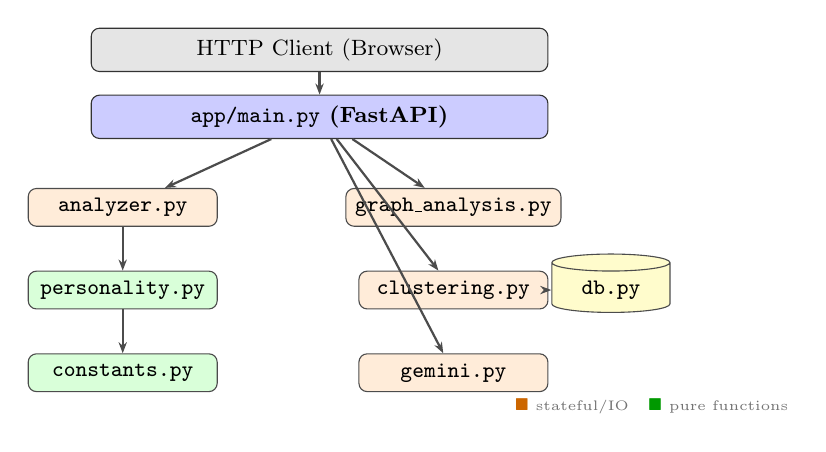
\begin{tikzpicture}[
  every node/.style={font=\footnotesize},
  client/.style={rectangle, rounded corners=3pt, draw=black!80,
                 fill=gray!20, minimum width=5.8cm, minimum height=0.55cm,
                 align=center},
  gateway/.style={rectangle, rounded corners=3pt, draw=black!80,
                  fill=blue!20, minimum width=5.8cm, minimum height=0.55cm,
                  align=center, font=\footnotesize\bfseries},
  modO/.style={rectangle, rounded corners=3pt, draw=black!70,
               fill=orange!15, minimum width=2.4cm, minimum height=0.48cm,
               align=center},
  modG/.style={rectangle, rounded corners=3pt, draw=black!70,
               fill=green!15, minimum width=2.4cm, minimum height=0.48cm,
               align=center},
  dbcyl/.style={cylinder, draw=black!70, fill=yellow!20,
                shape border rotate=90, aspect=0.22,
                minimum width=1.5cm, minimum height=0.48cm, align=center},
  arr/.style={-{Stealth[length=4pt]}, thick, black!70}
]
  % Top tier
  \node[client]  (client) at (0.5,  0   ) {HTTP Client (Browser)};
  \node[gateway] (main)   at (0.5, -0.85) {\texttt{app/main.py} (FastAPI)};

  % Left column: analyzer sub-chain (pure analytical path)
  \node[modO] (analyzer)    at (-2.0, -2.0) {\texttt{analyzer.py}};
  \node[modG] (personality) at (-2.0, -3.05) {\texttt{personality.py}};
  \node[modG] (constants)   at (-2.0, -4.10) {\texttt{constants.py}};

  % Right column: three independent domain modules
  \node[modO] (graph)      at ( 2.2, -2.0 ) {\texttt{graph\_analysis.py}};
  \node[modO] (clustering) at ( 2.2, -3.05) {\texttt{clustering.py}};
  \node[modO] (gemini)     at ( 2.2, -4.10) {\texttt{gemini.py}};

  % DB beside clustering
  \node[dbcyl] (db) at (4.2, -3.05) {\texttt{db.py}};

  % Arrows
  \draw[arr] (client) -- (main);
  \draw[arr] (main)   -- (analyzer);
  \draw[arr] (main)   -- (graph);
  \draw[arr] (main)   -- (clustering);
  \draw[arr] (main)   -- (gemini);
  \draw[arr] (analyzer)    -- (personality);
  \draw[arr] (personality) -- (constants);
  \draw[arr] (clustering)  -- (db);

  % Legend
  \node[font=\tiny, anchor=south west, text=black!55, align=left]
    at (2.85, -4.75)
    {\textcolor{orange!80!black}{$\blacksquare$}~stateful/I\kern0pt O\quad
     \textcolor{green!60!black}{$\blacksquare$}~pure functions};
\end{tikzpicture}
\caption{Module dependency graph. \texttt{main.py} is only HTTP entry
point. Orange = stateful/I/O modules; Green = pure functions that can be
tested in isolation.}
\label{fig:arch}
\end{figure}

\subsection{Technology Stack}

Table~\ref{tab:stack} is summarizing technology stack we used in our system.

\begin{table}[!t]
\caption{Technology Stack}
\label{tab:stack}
\centering
\tabletight
\begin{tabularx}{\columnwidth}{@{}lY@{}}
\toprule
\textbf{Layer} & \textbf{Technology} \\
\midrule
Web framework  & FastAPI + Uvicorn \\
Data processing & pandas $\geq$2.0, numpy $\geq$1.24, pyarrow $\geq$14 \\
Graph analysis  & NetworkX $\geq$3.0 \\
Clustering      & scikit-learn $\geq$1.3 \\
Distributed     & PySpark $\geq$3.5 (benchmark only) \\
AI analysis     & Google Gemini (gemini-2.5-flash) \\
Database        & SQLite (\texttt{benchmark.db}) \\
Containerization & Docker (\texttt{python:3.11-slim}) \\
Deployment      & AWS Elastic Beanstalk (Docker, \texttt{eu-west-1}) \\
Runtime         & Python 3.11+ \\
\bottomrule
\end{tabularx}
\end{table}

\subsection{Data Flow}

User is uploading one or more JSON files that produced by Spotify's Extended Streaming History export. \texttt{/analyze} endpoint is doing following steps:
\begin{enumerate}
  \item Parses and concatenates all uploaded files into flat record list.
  \item Calls \texttt{analyzer.analyze(records)} to produce core metrics
        dict.
  \item Calls \texttt{analyze\_listening\_graph(records)} for graph data.
  \item Optionally calls \texttt{analyze\_character(metrics)} for Gemini
        analysis.
  \item Serializes merged result to JSON and injects it into
        \texttt{dashboard.html} template via \texttt{render\_dashboard()}.
\end{enumerate}
All steps are happening inside single HTTP request; there is no background jobs or queues for primary analysis path. Fig.~\ref{fig:dataflow} is showing end-to-end request lifecycle.

\begin{figure}[ht]
\centering
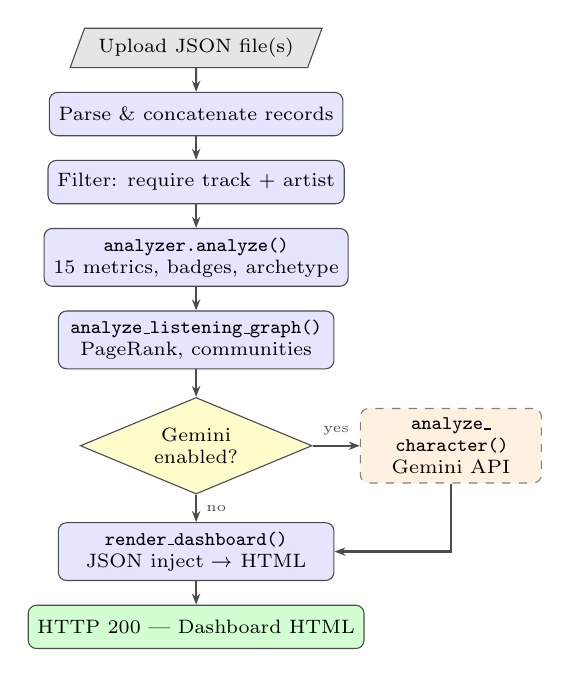
\begin{tikzpicture}[
  every node/.style={font=\scriptsize},
  flowstep/.style={rectangle, rounded corners=3pt, draw=black!70,
               fill=blue!10, minimum width=3.5cm, minimum height=0.55cm,
               align=center},
  io/.style={trapezium, trapezium left angle=70, trapezium right angle=110,
             draw=black!70, fill=gray!20, minimum width=3.2cm,
             minimum height=0.50cm, align=center},
  decision/.style={diamond, draw=black!70, fill=yellow!20,
                   minimum width=1.4cm, minimum height=0.8cm,
                   aspect=2.4, align=center},
  output/.style={rectangle, rounded corners=3pt, draw=black!70,
                 fill=green!18, minimum width=3.5cm, minimum height=0.55cm,
                 align=center},
  arr/.style={-{Stealth[length=4pt]}, thick, black!70},
  side/.style={rectangle, rounded corners=3pt, draw=black!50,
               fill=orange!12, minimum width=2.3cm, minimum height=0.50cm,
               align=center, dashed},
]
  \node[io]       (upload)   {Upload JSON file(s)};
  \node[flowstep, below=0.3cm of upload]  (parse)
        {Parse \& concatenate records};
  \node[flowstep, below=0.3cm of parse]   (filter)
        {Filter: require track + artist};
  \node[flowstep, below=0.3cm of filter]  (analyze)
        {\texttt{analyzer.analyze()}\\15 metrics, badges, archetype};
  \node[flowstep, below=0.3cm of analyze] (graph)
        {\texttt{analyze\_listening\_graph()}\\PageRank, communities};
  \node[decision, below=0.35cm of graph] (gemini_q)
        {Gemini\\enabled?};
  \node[flowstep, below=0.35cm of gemini_q] (render)
        {\texttt{render\_dashboard()}\\JSON inject → HTML};
  \node[output, below=0.3cm of render]  (resp)
        {HTTP 200 — Dashboard HTML};

  % Side branch: Gemini
  \node[side, right=0.6cm of gemini_q, text width=1.9cm] (gemini_call)
        {\texttt{analyze\_}\\\texttt{character()}\\Gemini API};

  % Arrows main flow
  \foreach \a/\b in {upload/parse, parse/filter, filter/analyze,
                      analyze/graph, graph/gemini_q, render/resp}
    \draw[arr] (\a) -- (\b);

  % Gemini branch
  \draw[arr] (gemini_q.east) -- node[above,font=\tiny]{yes}
             (gemini_call.west);
  \draw[arr] (gemini_call.south) |- (render.east);
  \draw[arr] (gemini_q.south) -- node[right,font=\tiny]{no}
             (render.north);

\end{tikzpicture}
\caption{End-to-end request lifecycle for \texttt{POST /analyze}
endpoint. All analytical steps are executing synchronously inside single
HTTP request. Gemini call is skipped when \texttt{GEMINI\_API\_KEY}
is absent or \texttt{SKIP\_GEMINI=1}. Optional SQLite write is
triggered separately via \texttt{POST /api/submit}.}
\label{fig:dataflow}
\end{figure}

\subsection{REST API}

Eight endpoints are exposed (Table~\ref{tab:api}).

\begin{table}[!t]
\caption{REST API Endpoints}
\label{tab:api}
\centering
\tabletight
\begin{tabularx}{\columnwidth}{@{}llY@{}}
\toprule
\textbf{Method} & \textbf{Path} & \textbf{Description} \\
\midrule
GET  & \texttt{/}                & Landing page \\
POST & \texttt{/analyze}         & Full dashboard from JSON upload \\
POST & \texttt{/api/submit}      & Submit metrics to benchmark DB \\
POST & \texttt{/api/percentiles} & Percentile ranking vs. pool \\
GET  & \texttt{/api/stats}       & Aggregate benchmark statistics \\
POST & \texttt{/api/graph}       & Graph analysis only \\
GET  & \texttt{/api/cluster}     & Cluster all benchmark DB users \\
GET  & \texttt{/api/health}      & Health check \\
\bottomrule
\end{tabularx}
\end{table}

% ─────────────────────────────────────────────────────────────────────────────
\section{Big Data Processing Pipeline}

\subsection{Three-Tier Architecture}

Datatify is implementing same analytical logic in three independent pipeline tiers, and each tier is targeting different scale regime:

\begin{enumerate}
  \item \textbf{Pure-Python tier} (\texttt{app/analyzer.py}): This is
        production request path. Single \texttt{for} loop over raw records
        is maintaining Python \texttt{defaultdict} accumulators. Time
        complexity is $O(N)$, memory is $O(D)$ where $D$ is number of distinct
        artists/tracks/time buckets. It is suitable for single-user exports
        ($N \leq 500\text{K}$).
  \item \textbf{Pandas tier} (\texttt{app/data\_pipeline.py}): Vectorized
        reference implementation. Records are loaded into \texttt{pd.DataFrame}
        and group-by aggregations are replacing Python accumulator loop. Memory
        layout is column-contiguous (NumPy arrays), which enabling
        SIMD-accelerated reductions. It is mirroring \texttt{analyzer.py}
        metric definitions exactly and serving as correctness cross-check
        for production path.
  \item \textbf{PySpark tier} (\texttt{app/spark\_pipeline.py}): Distributed
        implementation for horizontal scalability. Records are parallelized into
        RDD/DataFrame, partitioned across executors, and reduced via
        Spark SQL \texttt{groupBy} aggregations. Spark MLlib K-Means is used for
        distributed clustering. This tier is used only in \texttt{scripts/benchmark.py}
        and not in live request path.
\end{enumerate}

\begin{figure*}[t]
\centering
\resizebox{\textwidth}{!}{%
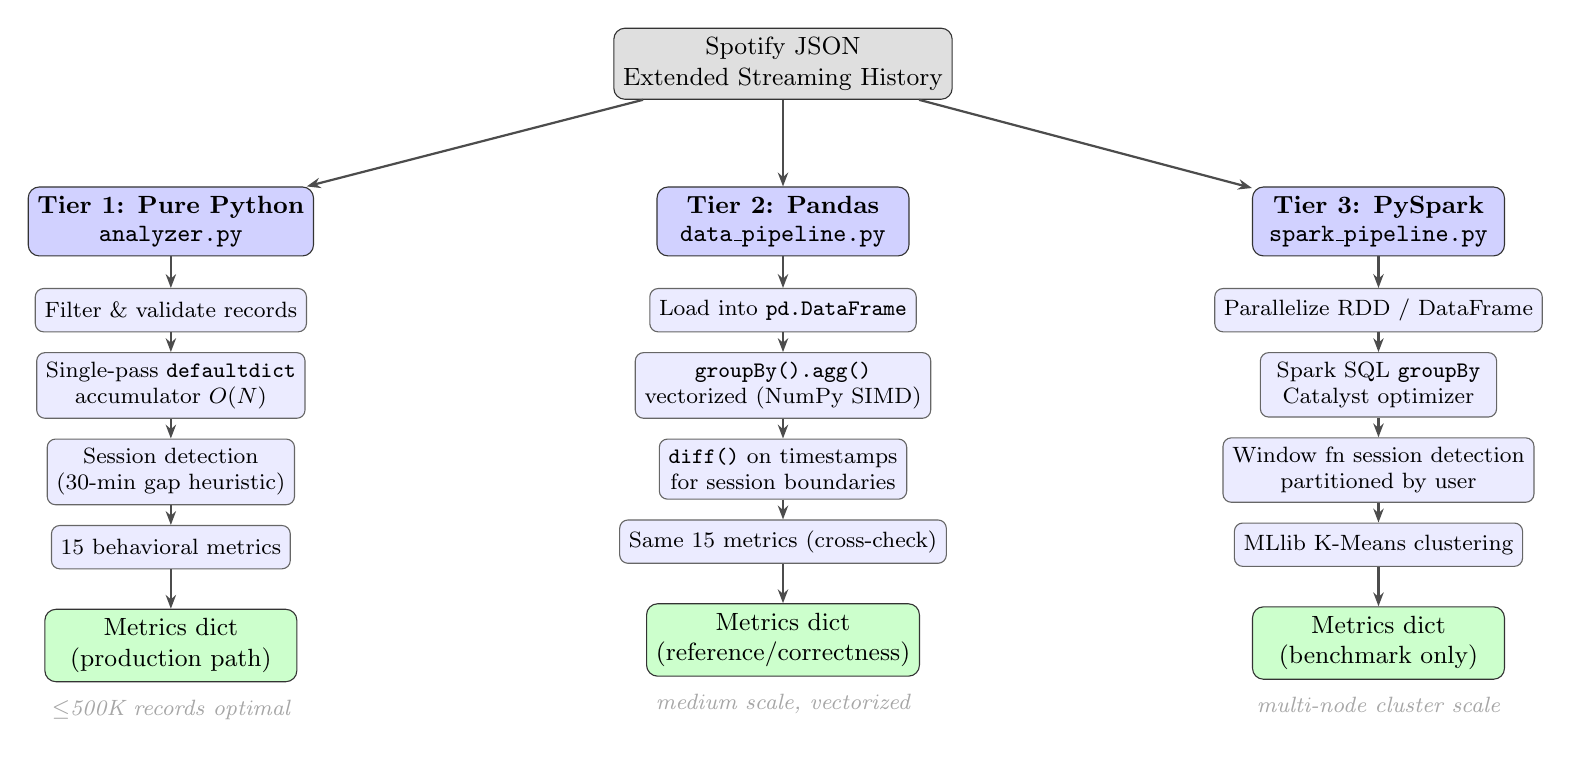
\begin{tikzpicture}[
  every node/.style={font=\small},
  input/.style={rectangle, rounded corners=4pt, draw=black!80,
                fill=gray!25, minimum width=3.2cm, minimum height=0.65cm,
                align=center},
  tier/.style={rectangle, rounded corners=4pt, draw=black!80,
               fill=blue!18, minimum width=3.2cm, minimum height=0.65cm,
               align=center},
  flowstep/.style={rectangle, rounded corners=3pt, draw=black!60,
               fill=blue!8, minimum width=3.0cm, minimum height=0.55cm,
               align=center, font=\footnotesize},
  output/.style={rectangle, rounded corners=4pt, draw=black!80,
                 fill=green!20, minimum width=3.2cm, minimum height=0.65cm,
                 align=center},
  label/.style={font=\footnotesize\itshape, text=gray!70},
  arr/.style={-{Stealth[length=5pt]}, thick, black!70},
  darr/.style={-{Stealth[length=5pt]}, thick, black!40, dashed}
]

  % ── Input node ────────────────────────────────────────────────
  \node[input] (input) {Spotify JSON\\Extended Streaming History};

  % ── Three tier headers ────────────────────────────────────────
  \node[tier, below left=1.1cm and 3.8cm of input]   (py_h)
        {\textbf{Tier 1: Pure Python}\\[-1pt]\texttt{analyzer.py}};
  \node[tier, below=1.1cm of input]                  (pd_h)
        {\textbf{Tier 2: Pandas}\\[-1pt]\texttt{data\_pipeline.py}};
  \node[tier, below right=1.1cm and 3.8cm of input]  (sp_h)
        {\textbf{Tier 3: PySpark}\\[-1pt]\texttt{spark\_pipeline.py}};

  % ── Tier 1 steps ──────────────────────────────────────────────
  \node[flowstep, below=0.4cm of py_h]  (py1) {Filter \& validate records};
  \node[flowstep, below=0.25cm of py1]  (py2) {Single-pass \texttt{defaultdict}\\accumulator $O(N)$};
  \node[flowstep, below=0.25cm of py2]  (py3) {Session detection\\(30-min gap heuristic)};
  \node[flowstep, below=0.25cm of py3]  (py4) {15 behavioral metrics};

  % ── Tier 2 steps ──────────────────────────────────────────────
  \node[flowstep, below=0.4cm of pd_h]  (pd1) {Load into \texttt{pd.DataFrame}};
  \node[flowstep, below=0.25cm of pd1]  (pd2) {\texttt{groupBy().agg()}\\vectorized (NumPy SIMD)};
  \node[flowstep, below=0.25cm of pd2]  (pd3) {\texttt{diff()} on timestamps\\for session boundaries};
  \node[flowstep, below=0.25cm of pd3]  (pd4) {Same 15 metrics (cross-check)};

  % ── Tier 3 steps ──────────────────────────────────────────────
  \node[flowstep, below=0.4cm of sp_h]  (sp1) {Parallelize RDD / DataFrame};
  \node[flowstep, below=0.25cm of sp1]  (sp2) {Spark SQL \texttt{groupBy}\\Catalyst optimizer};
  \node[flowstep, below=0.25cm of sp2]  (sp3) {Window fn session detection\\partitioned by user};
  \node[flowstep, below=0.25cm of sp3]  (sp4) {MLlib K-Means clustering};

  % ── Output collectors ─────────────────────────────────────────
  \node[output, below=0.5cm of py4] (out_py)
        {Metrics dict\\(production path)};
  \node[output, below=0.5cm of pd4] (out_pd)
        {Metrics dict\\(reference/correctness)};
  \node[output, below=0.5cm of sp4] (out_sp)
        {Metrics dict\\(benchmark only)};

  % ── Arrows: input → tier headers ─────────────────────────────
  \draw[arr] (input) -- (py_h);
  \draw[arr] (input) -- (pd_h);
  \draw[arr] (input) -- (sp_h);

  % ── Arrows: within tiers ─────────────────────────────────────
  \foreach \a/\b in {py_h/py1, py1/py2, py2/py3, py3/py4, py4/out_py,
                      pd_h/pd1, pd1/pd2, pd2/pd3, pd3/pd4, pd4/out_pd,
                      sp_h/sp1, sp1/sp2, sp2/sp3, sp3/sp4, sp4/out_sp}
    \draw[arr] (\a) -- (\b);

  % ── Scale labels ─────────────────────────────────────────────
  \node[label, below=0.1cm of out_py] {$\leq$500K records optimal};
  \node[label, below=0.1cm of out_pd] {medium scale, vectorized};
  \node[label, below=0.1cm of out_sp] {multi-node cluster scale};

\end{tikzpicture}%
}
\caption{Three-tier big data processing pipeline. All three tiers are
implementing identical analytical logic and producing same 15 behavioral
metrics. Tier 1 (pure Python) is production request path; Tier 2 (Pandas)
is serving as correctness cross-check; Tier 3 (PySpark) is targeting
distributed multi-user deployments and used only in scalability benchmark.}
\label{fig:pipeline}
\end{figure*}

\subsection{Data Volume Characteristics}

Spotify Extended Streaming History export is big data artefact at boundary of single-node and distributed processing:
\begin{itemize}
  \item \textbf{Typical export}: 50\,K--200\,K records for 3--5 year history.
  \item \textbf{Heavy user export}: up to 500\,K records.
  \item \textbf{Synthetic benchmark}: 100\,K--2\,M records generated by
        \texttt{scripts/synthetic\_data.py} for stress-testing all three tiers.
  \item \textbf{Multi-user population}: millions of records if aggregated across
        voluntary contributors---this is scale where PySpark is becoming advantageous.
\end{itemize}

\subsection{Synthetic Data Generation}

Benchmark script \texttt{scripts/synthetic\_data.py} is generating realistic Spotify record distributions: artist play-counts are following Zipf distribution (small set of artists is dominating, which is matching real listening data), timestamps are following Poisson arrival process with circadian modulation (higher density during evening hours), and skip/shuffle flags are sampled from configurable Bernoulli distributions. In this way we can do controlled scaling experiments at record counts which are beyond typical real-world exports.

\subsection{PySpark Implementation}

PySpark pipeline (\texttt{spark\_pipeline.py}) is mirroring analytical logic of \texttt{analyzer.py} using distributed primitives:

\begin{itemize}
  \item Records are loaded as Spark DataFrame with inferred schema.
  \item Artist and track aggregations are using \texttt{df.groupBy(...).agg(...)},
        which Spark is optimizing via Catalyst query planner and Tungsten
        execution engine.
  \item Session detection is using window function
        \texttt{Window.partitionBy().orderBy("ts")} with lag-based gap
        computation, and this is replacing Python sort-and-scan loop.
  \item K-Means clustering is using \texttt{pyspark.ml.clustering.KMeans} with
        same $k$-means++ initialization as scikit-learn implementation,
        operating on \texttt{VectorAssembler}-transformed feature columns.
  \item Results are collected back to driver with \texttt{df.collect()}
        for JSON serialization.
\end{itemize}

Spark context is initialized with local master (\texttt{SparkSession.builder.master("local[*]")}) for single-node benchmarking; in real distributed deployment, replacing \texttt{"local[*]"} with cluster URL is enough to enable horizontal scaling across multiple nodes without any code changes.

\subsection{Pandas Implementation}

Pandas pipeline (\texttt{data\_pipeline.py}) is implementing same logic using vectorized DataFrame operations via \texttt{compute\_metrics\_pandas(df)}:

\begin{itemize}
  \item Timestamps are parsed with \texttt{pd.to\_datetime()} which is using
        NumPy's datetime64 representation for efficient sorting and arithmetic.
  \item Aggregations are using \texttt{groupby().agg()} on columnar arrays,
        and this is enabling SIMD-accelerated summation.
  \item Shannon entropy is computed as \texttt{numpy} reduction over
        play-count column.
  \item Session detection is using \texttt{diff()} on sorted timestamps and
        boolean masking to find gap boundaries without explicit loop.
\end{itemize}

% ─────────────────────────────────────────────────────────────────────────────
\section{Core Analysis Engine}

\subsection{Input Schema}

Each streaming record is JSON object with four required fields: \texttt{ts} (ISO-8601 UTC timestamp), \texttt{ms\_played} (integer milliseconds), \texttt{master\_metadata\_track\_name}, and \texttt{master\_metadata\_album\_artist\_name}. Nine additional fields---album name, skip flag, shuffle flag, start/end reasons, country code, platform, offline flag, and incognito mode---are treated as optional enrichment columns. Records that missing both required track and artist fields are silently filtered before analysis.

\subsection{Single-Pass Aggregation}

Function \texttt{\_aggregate\_records(tracks)} is performing single iteration over filtered record list, and maintaining defaultdict accumulators for artists, tracks, albums, year/month/hour/weekday/platform/country buckets, play-reason counters, skip-related sub-counts, and first-listen maps. By accumulating everything in one pass, time complexity is $O(N)$ where $N$ is number of records, and this is avoiding repeated scans for each dimension.

Accumulators that are returned include:
\begin{itemize}
  \item \texttt{artists}: per-artist total milliseconds, play count, skip count.
  \item \texttt{songs}: per-(track, artist) pair play count and total ms.
  \item \texttt{by\_year/month/hour/weekday}: temporal bucketing.
  \item \texttt{by\_platform}: categorized as \textit{Mobil}, \textit{Web},
        or \textit{Masaüstü} via string inspection of raw platform field.
  \item \texttt{skipped\_count}, \texttt{completed\_count},
        \texttt{early\_skip\_count}, \texttt{focus\_play\_count}: behavioral
        counters that are used directly as metric numerators.
  \item \texttt{first\_listen}: first timestamp per artist and per
        (track, artist) pair, used for novelty and loyalty badge computations.
\end{itemize}

\subsection{Session Detection}

Sessions are computed by \texttt{\_compute\_sessions(tracks)}, which is sorting records by timestamp and grouping consecutive plays separated by fewer than $G = 30$\,min. Formally, play $p_{i+1}$ is starting new session if
\begin{equation}
  \mathrm{start}(p_{i+1}) - \mathrm{end}(p_i) > G,
\end{equation}
where $\mathrm{start}(p) = \texttt{ts}(p) - \texttt{ms\_played}(p)$ (reconstructed start time) and $\mathrm{end}(p) = \texttt{ts}(p)$ (record timestamp is end of playback). Function is returning session list, count, and average session duration in hours. 30-minute boundary is consistent with session-segmentation conventions adopted in music streaming research~\cite{brost2019sessions}. Constant $G$ is centralized in \texttt{constants.SESSION\_GAP\_MINUTES} so all modules are sharing same boundary condition.

\subsection{Timezone Correction}

Spotify timestamps are UTC. Circadian analysis require local-time hours. Dominant country is determined by country code that accumulating most milliseconds. Offset lookup table \texttt{TZ\_OFFSETS} is mapping 30 country codes to integer UTC offsets; Turkish users (country code \texttt{TR}) are receiving offset +3. Night listening hours (00:00--05:59 local) are computed by shifting UTC hour buckets by detected offset modulo 24.

\subsection{Behavioral Metrics}

Fifteen normalized metrics are derived from aggregated accumulators (Table~\ref{tab:metrics}). Some important ones are:

\textbf{Artist Diversity Entropy}~\cite{shannon1948mathematical} is Shannon entropy of artist play-count distribution:
\begin{equation}
  H = -\sum_{a} \frac{c_a}{N} \log_2 \frac{c_a}{N},
\end{equation}
where $c_a$ is play count for artist $a$ and $N$ is total play count. Higher entropy is indicating that user is listening more broad and uniform distribution of artists.

\textbf{Habit Loop Score} is capturing consecutive-pair repetition:
\begin{equation}
  \text{HLS} = \frac{|\{(p_i, p_{i+1}) : \mathrm{count}(p_i, p_{i+1}) > 1\}|}{N - 1} \times 100,
\end{equation}
where $(p_i, p_{i+1})$ is ordered (track, artist) pair and counts are accumulated across sorted timeline.

\textbf{Monthly Novelty Rate} is averaging fraction of new tracks (first listens) per month:
\begin{equation}
  \text{NVR} = \frac{1}{|M|} \sum_{m \in M} \frac{\text{new\_tracks}(m)}{\text{plays}(m)} \times 100,
\end{equation}
where $M$ is set of months that present in listening history.

\begin{table}[!t]
\caption{The 15 Behavioral Metrics}
\label{tab:metrics}
\centering
\scriptsize
\setlength{\tabcolsep}{2.5pt}
\renewcommand{\arraystretch}{1.12}
\begin{tabularx}{\columnwidth}{@{}p{4.32cm}Y@{}}
\toprule
\textbf{Metric Key} & \textbf{Definition} \\
\midrule
\texttt{impatience\_score\_pct}          & \% plays that were skipped \\
\texttt{completion\_rate\_pct}           & \% plays ending with ``endplay'' \\
\texttt{exploration\_score}              & $100 \times \text{unique tracks} / \text{total plays}$ \\
\texttt{artist\_diversity\_entropy}      & Shannon entropy of artist play counts \\
\texttt{early\_skip\_rate\_pct}          & \% skips where ms\_played $<$ 30s \\
\texttt{listening\_intensity\_h\_per\_day} & Total hours / calendar days \\
\texttt{night\_listening\_ratio\_pct}    & \% ms in local 00:00–05:59 \\
\texttt{mobile\_usage\_ratio\_pct}       & \% ms on mobile platform \\
\texttt{focus\_session\_score\_pct}      & \% non-skipped plays $\geq$ 4\,min \\
\texttt{music\_novelty\_rate\_pct}       & Avg.\ \% new tracks per month \\
\texttt{artist\_loyalty\_score\_pct}     & \% plays by top-10 artists \\
\texttt{habit\_loop\_score\_pct}         & \% repeated (track, artist) consecutive pairs \\
\texttt{listening\_fragmentation\_index} & Skipped plays / session count \\
\texttt{total\_hours}                    & Total listening hours \\
\texttt{shuffle\_pct}                    & \% plays in shuffle mode \\
\bottomrule
\end{tabularx}
\end{table}

% ─────────────────────────────────────────────────────────────────────────────
\section{Personality Profiling and Gamification}

\subsection{Radar Chart}

Six-axis radar chart is mapping selected metrics to normalized 0--100 values:
\begin{align*}
  \text{Patience}   &= 100 - \text{impatience\_score\_pct}, \\
  \text{Discovery}  &= \min(\text{exploration\_score} \times 5,\; 100), \\
  \text{Loyalty}    &= \min(\text{artist\_loyalty\_score\_pct} \times 5,\; 100), \\
  \text{Focus}      &= \min(\text{focus\_session\_score\_pct} \times 5,\; 100), \\
  \text{Diversity}  &= \min(\text{artist\_diversity\_entropy} \times 8,\; 100), \\
  \text{Night Owl}  &= \min(\text{night\_listening\_ratio\_pct} \times 4,\; 100).
\end{align*}
Scaling constants are chosen empirically so typical listener is scoring between 20 and 80 on each axis, and this is providing good visual separation. Fig.~\ref{fig:radar} is showing two contrasting listener profiles on six-axis radar.

\begin{figure}[ht]
\centering
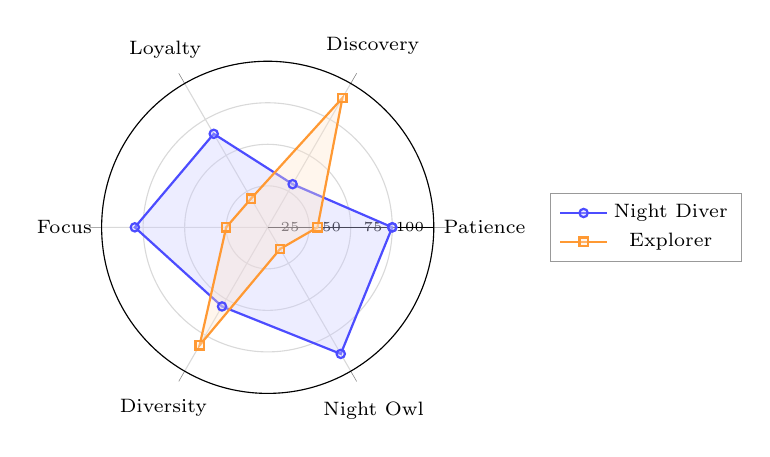
\begin{tikzpicture}
\begin{polaraxis}[
  width=5.8cm, height=5.8cm,
  xtick={0,60,120,180,240,300},
  xticklabels={Patience, Discovery, Loyalty, Focus, Diversity, Night Owl},
  xticklabel style={font=\scriptsize},
  ymin=0, ymax=100,
  ytick={25,50,75,100},
  yticklabel style={font=\tiny, anchor=east},
  ytick style={draw=none},
  yticklabels={25,50,75,100},
  grid=both,
  grid style={draw=gray!30, line width=0.4pt},
  legend style={at={(1.35,0.5)}, anchor=west,
                font=\scriptsize, draw=black!40, fill=white},
  legend entries={Night Diver, Explorer},
]
  % Night Diver: high patience, low discovery, medium loyalty,
  %              high focus, medium diversity, very high night owl
  \addplot[thick, color=blue!70, fill=blue!20, fill opacity=0.35, mark=*,
           mark size=1.5pt]
    coordinates {
      (0,75) (60,30) (120,65) (180,80) (240,55) (300,88) (360,75)
    };
  % Restless Explorer: low patience, very high discovery, low loyalty,
  %                    low focus, high diversity, low night owl
  \addplot[thick, color=orange!80, fill=orange!20, fill opacity=0.35,
           mark=square*, mark size=1.5pt]
    coordinates {
      (0,30) (60,90) (120,20) (180,25) (240,82) (300,15) (360,30)
    };
\end{polaraxis}
\end{tikzpicture}
\caption{Six-axis radar chart for two contrasting archetypes. \textit{Night
Diver} (blue) is scoring high on Patience, Focus, and Night Owl axes.
\textit{Restless Explorer} (orange) is dominating Discovery and Diversity
but scoring low on Patience and Loyalty.}
\label{fig:radar}
\end{figure}

\subsection{Listener Archetypes}

Seven deterministic archetype rules are evaluated in order against metric vector (Table~\ref{tab:archetypes}). First matching rule is determining archetype; if none is matched, user is classified as \textit{The Balanced Listener}. Rule evaluation is $O(1)$ per user because all inputs are scalars that already computed during aggregation. Threshold values are placed at empirical 75th-percentile boundary of each relevant metric across benchmark pool, and this is ensuring that each specialized archetype is capturing most pronounced behavioral patterns before default fallback is applied.

\begin{table}[!t]
\caption{Archetype Classification Rules}
\label{tab:archetypes}
\centering
\tabletight
\begin{tabularx}{\columnwidth}{@{}p{2.7cm}Y@{}}
\toprule
\textbf{Archetype} & \textbf{Rule} \\
\midrule
The Night Diver       & Night $>$ 25\% \textbf{and} Focus $>$ 10\% \\
The Restless Explorer & Impatience $>$ 40\% \textbf{and} Exploration $>$ 12 \\
The Loyal Guardian    & Loyalty $>$ 18\% \textbf{and} Novelty $<$ 7\% \\
The Eclectic Mind     & Entropy $>$ 10 \textbf{and} Exploration $>$ 8 \\
The Deep Listener     & Focus $>$ 12\% \textbf{and} Impatience $<$ 25\% \\
The Picky Repeater    & Impatience $>$ 35\% \textbf{and} Novelty $<$ 6\% \\
The Midnight Wanderer & Night $>$ 20\% \textbf{and} Entropy $>$ 9 \\
The Balanced Listener & Default (no rule matched) \\
\bottomrule
\end{tabularx}
\end{table}

\subsection{Level System}

Gamification level is derived from total listening hours (Table~\ref{tab:levels}). Experience points are computed as:
\begin{equation}
  \text{XP} = \lfloor \text{total\_hours} \times 10 \rfloor + \text{badges\_earned} \times 50,
\end{equation}
and this is combining continuous engagement (hours) with discrete achievement bonuses (badges). Multiplicative constants are weighting badge acquisition at approximately equivalent of five hours of listening each.

\begin{table}[!t]
\caption{Level Thresholds}
\label{tab:levels}
\centering
\tabletight
\begin{tabular}{cll}
\toprule
\textbf{Level} & \textbf{Title} & \textbf{Min.\ Hours} \\
\midrule
1  & Newbie       & 0 \\
2  & Casual       & 50 \\
3  & Listener     & 200 \\
4  & Enthusiast   & 500 \\
5  & Devotee      & 1\,000 \\
6  & Addict       & 1\,500 \\
7  & Obsessed     & 2\,000 \\
8  & Maniac       & 2\,500 \\
9  & Legendary    & 3\,000 \\
10 & Mythic       & 4\,000 \\
11 & Transcendent & 5\,000 \\
\bottomrule
\end{tabular}
\end{table}

\subsection{Achievement Badges}

Fifteen binary achievement badges are evaluated in \texttt{compute\_badges()}. Each badge have deterministic boolean predicate over metric vector and summary report. Some example badges are:
\begin{itemize}
  \item \textit{Marathon Listener}: single session $\geq$ 4\,h.
  \item \textit{Explorer}: $\geq$1\,000 unique artists.
  \item \textit{Loyal Fan}: $\geq$1 artist followed for $\geq$5 years with
        $\geq$20 plays.
  \item \textit{Centurion}: $\geq$100\,000 total plays.
  \item \textit{World Traveler}: streams detected from $\geq$3 countries.
  \item \textit{Creature of Habit}: habit-loop score $>$ 10\%.
\end{itemize}

% ─────────────────────────────────────────────────────────────────────────────
\section{Artist Transition Graph Analysis}

\subsection{Graph Construction}

Listening history is modeled as weighted directed graph $G = (V, E, w)$ where each node $v \in V$ is artist and directed edge $(a_i, a_j) \in E$ exist if artist $a_j$ is played within 30\,min of artist $a_i$ in chronological order. Edge weight $w(a_i, a_j)$ is counting number of such consecutive occurrences. Self-loops (same artist back-to-back within session) are kept because they are capturing single-artist intensive listening episodes.

Construction pipeline is proceeding as following:
\begin{enumerate}
  \item \texttt{\_parse\_artist\_timeline(records)}: filter records,
        extract (timestamp, artist) pairs, report
        \texttt{dropped\_no\_artist} and \texttt{dropped\_bad\_ts}
        diagnostics.
  \item Sort by timestamp.
  \item Iterate consecutive pairs; emit edge if gap $\leq G$.
  \item Build \texttt{nx.DiGraph} from edge-weight dictionary.
\end{enumerate}
Every call to \texttt{analyze\_listening\_graph()} is returning \texttt{parse\_diagnostics} dict inside \texttt{summary} key, and this providing full visibility into data quality to callers.

Fig.~\ref{fig:graph} is showing schematic artist-transition graph with two detected communities and PageRank-ranked central nodes.

\begin{figure}[ht]
\centering
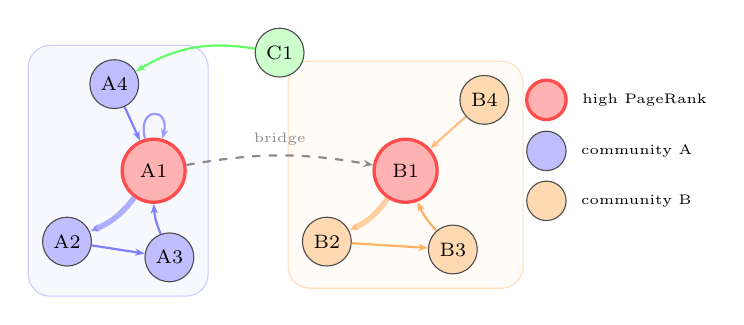
\begin{tikzpicture}[
  every node/.style={font=\scriptsize},
  artist/.style={circle, draw=black!70, minimum size=0.62cm,
                 align=center, inner sep=1pt},
  comA/.style={artist, fill=blue!25},
  comB/.style={artist, fill=orange!30},
  comC/.style={artist, fill=green!20},
  hipr/.style={artist, fill=red!30, minimum size=0.80cm,
               draw=red!70, line width=1.2pt},
  arr/.style={-{Stealth[length=3.5pt]}, thick},
  warr/.style={-{Stealth[length=3.5pt]}, line width=2.0pt, opacity=0.5},
]
  % ── Community A (blue) ───────────────────────────
  \node[hipr]  (A1) at (0,    0)    {A1};   % high PageRank gateway
  \node[comA]  (A2) at (-1.1, -0.9) {A2};
  \node[comA]  (A3) at ( 0.2, -1.1) {A3};
  \node[comA]  (A4) at (-0.5,  1.1) {A4};

  % ── Community B (orange) ─────────────────────────
  \node[hipr]  (B1) at ( 3.2,  0)   {B1};
  \node[comB]  (B2) at ( 2.2, -0.9) {B2};
  \node[comB]  (B3) at ( 3.8, -1.0) {B3};
  \node[comB]  (B4) at ( 4.2,  0.9) {B4};

  % ── Isolated node (green) ────────────────────────
  \node[comC]  (C1) at ( 1.6,  1.5) {C1};

  % ── Intra-community edges (A) ─────────────────────
  \draw[warr, blue!60]   (A1) to[bend left=15]  (A2);
  \draw[arr,  blue!50]   (A2) -- (A3);
  \draw[arr,  blue!50]   (A3) to[bend left=10]  (A1);
  \draw[arr,  blue!50]   (A4) -- (A1);
  \draw[arr,  blue!40]   (A1) to[loop above, looseness=5] (A1);  % self-loop

  % ── Intra-community edges (B) ─────────────────────
  \draw[warr, orange!70] (B1) to[bend left=15]  (B2);
  \draw[arr,  orange!60] (B2) -- (B3);
  \draw[arr,  orange!60] (B3) to[bend left=10]  (B1);
  \draw[arr,  orange!50] (B4) -- (B1);

  % ── Cross-community bridge ────────────────────────
  \draw[arr,  black!45, dashed] (A1) to[bend left=10] node[above,font=\tiny]{bridge} (B1);

  % ── Isolated component ───────────────────────────
  \draw[arr,  green!60]  (C1) to[bend right=20] (A4);

  % ── Legend ───────────────────────────────────────
  \node[hipr,  right=0.2cm of B4, minimum size=0.5cm] (lh) {};
  \node[comA,  below=0.12cm of lh, minimum size=0.5cm] (la) {};
  \node[comB,  below=0.12cm of la, minimum size=0.5cm] (lb) {};
  \node[font=\tiny, right=0.06cm of lh] {high PageRank};
  \node[font=\tiny, right=0.06cm of la] {community A};
  \node[font=\tiny, right=0.06cm of lb] {community B};

  % ── Community boundary annotations ───────────────
  \begin{scope}[on background layer]
    \node[draw=blue!40, fill=blue!5, rounded corners=8pt, opacity=0.5,
          fit=(A1)(A2)(A3)(A4), inner sep=5pt] {};
    \node[draw=orange!50, fill=orange!5, rounded corners=8pt, opacity=0.5,
          fit=(B1)(B2)(B3)(B4), inner sep=5pt] {};
  \end{scope}

\end{tikzpicture}
\caption{Schematic artist-transition graph $G$. Nodes are artists;
directed edge $A_i \to A_j$ is existing when $A_j$ is following $A_i$
within 30-min session. Bold-bordered nodes have high PageRank (gateway
artists). Shaded regions are label-propagation communities. Dashed edge
is cross-community bridge. Self-loop on A1 is indicating single-artist
repeat sessions.}
\label{fig:graph}
\end{figure}

\subsection{PageRank Centrality}

PageRank \cite{page1999pagerank} is computed on $G$ with damping factor $\alpha = 0.85$, edge weights used as transition probabilities, convergence tolerance $\epsilon = 10^{-7}$, and maximum 200 iterations. Artist with high PageRank score mean that user is frequently transitioning \emph{to} that artist from many other contexts, and this is distinguishing gateway artists from those that listened only in isolation.

\subsection{Community Detection}

Label-propagation algorithm \cite{raghavan2007near} is applied to undirected projection of $G$ (edge weights preserved, direction dropped). Starting from random label assignment, each node is iteratively adopting label held by plurality of its weighted neighbors until convergence. Result is partition of artists into co-listened communities, ranked by total weighted degree. Top 10 communities are returned with size, aggregate weight, and up to 8 representative artists per community.

\subsection{Connected Components}

Weakly connected components of $G$ are revealing ``listening islands''---groups of artists that user is listening in separate, non-overlapping temporal contexts. Large number of small components is suggesting highly segmented listening behavior; single dominant component is suggesting fluid cross-genre exploration.

\subsection{Visualization Subgraph}

Force-directed frontend visualization is built from trimmed subgraph containing top-60 nodes by PageRank score, and only intra-group edges are retained with self-loops removed. Up to $\max(80, 2 \times 60) = 120$ highest-weight edges are included to prevent rendering overload in browser.

% ─────────────────────────────────────────────────────────────────────────────
\section{Listener Clustering}

\subsection{Feature Vector}

Each anonymous benchmark submission is represented as 15-dimensional vector using exactly keys in \texttt{METRIC\_KEYS} (Table~\ref{tab:metrics}). Two keys are originating from summary report rather than metrics namespace: \texttt{total\_hours} is mapping from \texttt{bizim\_rapor.toplam\_saat} and \texttt{shuffle\_pct} from \texttt{bizim\_rapor.shuffle\_orani\_pct}. This mapping is encapsulated in \texttt{db.extract\_metric\_vector()}, and this ensuring single authoritative translation from analysis output to cluster input.

\subsection{Preprocessing and Optimal-\texorpdfstring{$k$}{k} Selection}

Feature vectors are standardized using \texttt{sklearn.StandardScaler} (zero mean, unit variance) so that high-magnitude metrics like \texttt{total\_hours} are not dominating distance function.

Optimal cluster count is selected by \texttt{find\_optimal\_k()} using following procedure for each $k \in [k_{\min}, k_{\max}]$:
\begin{enumerate}
  \item Fit \texttt{KMeans(n\_clusters=k, init="k-means++", n\_init=10,
        random\_state=42)}.
  \item Record inertia (within-cluster sum of squares).
  \item Compute silhouette score \cite{rousseeuw1987silhouettes}.
\end{enumerate}
Final $k$ is chosen as $\arg\max_k \text{silhouette}(k)$ (Fig.~\ref{fig:silhouette}). Range $k \in [2, 8]$ was determined empirically: silhouette scores are becoming plateau beyond $k = 6$ on benchmark pools with more than 100 submissions (additional clusters are fragmenting rather than separating behaviors), and $k_{\min} = 2$ is preventing degenerate single-group results. If pool is containing fewer than four submissions, endpoint is returning \texttt{status: "insufficient\_data"} without attempting to cluster.

\begin{figure}[ht]
\centering
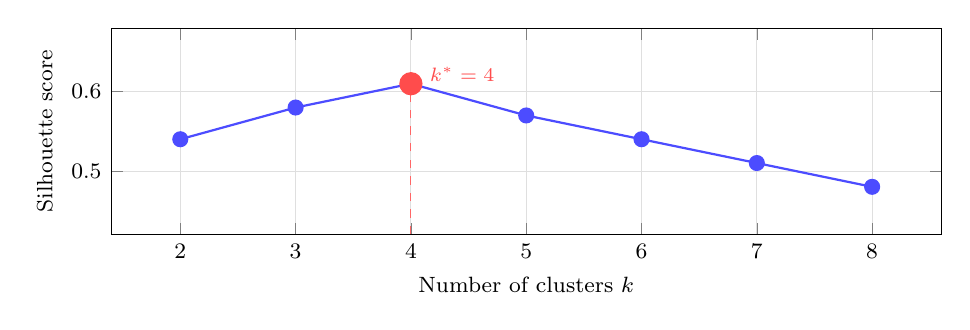
\begin{tikzpicture}
\begin{axis}[
  width=\columnwidth,
  height=4.2cm,
  xlabel={Number of clusters $k$},
  ylabel={Silhouette score},
  xlabel style={font=\footnotesize},
  ylabel style={font=\footnotesize},
  tick label style={font=\footnotesize},
  xtick={2,3,4,5,6,7,8},
  ymin=0.42, ymax=0.68,
  grid=major,
  grid style={line width=0.3pt, draw=gray!25},
  mark size=2.5pt,
]
  \addplot[color=blue!70, mark=*, thick]
    coordinates {(2,0.54)(3,0.58)(4,0.61)(5,0.57)(6,0.54)(7,0.51)(8,0.48)};
  \addplot[only marks, mark=*, mark size=4pt, color=red!70, forget plot]
    coordinates {(4,0.61)};
  \draw[dashed, red!60] (axis cs:4,0.42) -- (axis cs:4,0.61);
  \node[font=\scriptsize, text=red!70, anchor=south west]
    at (axis cs:4.08,0.60) {$k^*=4$};
\end{axis}
\end{tikzpicture}
\caption{Silhouette score vs.\ $k$ for K-Means++ on representative
benchmark pool of 200 submissions. Score is peaking at $k^*=4$; plateau
and decline beyond $k=5$ is confirming that $k_{\max}=8$ is safe upper
bound.}
\label{fig:silhouette}
\end{figure}

\subsection{Cluster Labeling}

Cluster centroids are inverse-transformed to original feature scale and inspected by \texttt{label\_cluster(centroid)}, which is applying priority cascade of seven heuristic rules (Table~\ref{tab:clabels}) to assign human-readable cluster name. Unlabeled clusters are falling back to \textit{Balanced Listeners}.

\begin{table}[!t]
\caption{Cluster Labeling Rules}
\label{tab:clabels}
\centering
\tabletight
\begin{tabularx}{\columnwidth}{@{}p{2.6cm}Y@{}}
\toprule
\textbf{Label} & \textbf{Centroid Condition} \\
\midrule
Night Explorers     & Night $>$ 25\% \textbf{and} Exploration $>$ 10 \\
Impatient Skippers  & Impatience $>$ 35\% \textbf{and} Exploration $>$ 12 \\
Loyal Repeaters     & Loyalty $>$ 18\% \textbf{and} Novelty $<$ 7\% \\
Deep Listeners      & Focus $>$ 12\% \textbf{and} Impatience $<$ 25\% \\
Heavy Discoverers   & Intensity $>$ 3\,h/day \textbf{and} Exploration $>$ 8 \\
Late Night Listeners & Night $>$ 20\% \\
Devoted Fans        & Loyalty $>$ 25\% \\
Balanced Listeners  & Default \\
\bottomrule
\end{tabularx}
\end{table}

\subsection{User Placement}

When current user's vector is provided, it is scaled with fitted \texttt{StandardScaler}, assigned to cluster by fitted \texttt{KMeans} model, and returned with cluster label, size, and share percentage. In this way user can see which behavioral cohort they belong to relative to anonymous benchmark pool.

% ─────────────────────────────────────────────────────────────────────────────
\section{AI Character Analysis}

\subsection{Gemini Integration}

\texttt{app/gemini.py} module is encapsulating entire AI subsystem without FastAPI dependency. Public entry point is \texttt{analyze\_character(metrics: dict) -> dict | None}, which is returning structured Turkish-language character portrait or \texttt{None} if analysis is failing or skipped.

\subsection{Model Fallback Chain}

Three Gemini model variants are tried in order: \texttt{gemini-2.5-flash} $\to$ \texttt{gemini-2.0-flash} $\to$ \texttt{gemini-flash-latest}. For each model, up to two attempts (\texttt{GEMINI\_MAX\_ATTEMPTS=2}) are made with per-call timeout of 25\,s (\texttt{GEMINI\_TIMEOUT=25s}) and total budget of 60\,s across all models and attempts (\texttt{GEMINI\_BUDGET=60s}).

\subsection{Rate Limiting}

Free-tier Gemini accounts are limited to 4 requests per minute (RPM). Module is implementing sliding-window RPM limiter: timestamp deque is tracking recent call times; each new call is checking whether window is full and sleeping minimal necessary duration before proceeding. This is allowing production deployment to operate safely on free tier without external rate-limiting infrastructure.

\subsection{Error Classification}

HTTP errors are inspected by \texttt{\_classify\_error(exc)}, which is returning tuple \texttt{(code, retry\_after, kind)} distinguishing: rate-limit errors (429, kind \texttt{rate\_limit}), server errors (5xx, kind \texttt{server\_error}), and client errors (4xx, kind \texttt{client\_error}). Only rate-limit and server errors are triggering retries; client errors are aborting immediately to avoid wasting budget.

\subsection{Prompt Design}

Prompt is constructing compact behavioral summary from metric vector (top artists, total hours, archetype, metric highlights) and instructing Gemini to produce structured response with five fields: \texttt{title}, \texttt{summary}, \texttt{traits} (list), \texttt{insights} (list), and \texttt{prediction}. Turkish language constraint is enforced in system instruction to ensure output is localized consistently with dashboard.

% ─────────────────────────────────────────────────────────────────────────────
\section{Scalability Benchmark}
\label{sec:benchmark}

\subsection{Experimental Setup}

For characterizing performance of three pipeline tiers at different data volumes, we generated synthetic Spotify records using \texttt{scripts/synthetic\_data.py} with Zipf artist distribution and Poisson-modulated timestamp arrivals at four scales: 100\,K, 500\,K, 1\,M, and 2\,M records. Wall-clock times are measured using Python's \texttt{time.perf\_counter()} and single warm-up run was discarded. All runs executed on same hardware under identical conditions. PySpark is configured with \texttt{local[*]} (all available cores) to give it best possible single-node performance.

\subsection{Results}

Table~\ref{tab:bench} is reporting wall-clock processing times in seconds. Fig.~\ref{fig:bench} is visualizing grouped bar comparison and Fig.~\ref{fig:bench_line} is showing log-scale line plot that used to confirm linear growth for Python and Pandas.

\begin{table}[!t]
\caption{Wall-Clock Processing Time (seconds)}
\label{tab:bench}
\centering
\tabletight
\begin{tabular}{rrrr}
\toprule
\textbf{Records} & \textbf{Pure Python} & \textbf{Pandas} & \textbf{PySpark} \\
\midrule
100\,000    & 0.753  & 0.674  & 9.137  \\
500\,000    & 3.815  & 3.477  & 13.470 \\
1\,000\,000 & 7.815  & 8.574  & 24.417 \\
2\,000\,000 & 17.327 & 13.987 & 50.744 \\
\bottomrule
\end{tabular}
\end{table}

\begin{figure}[ht]
\centering
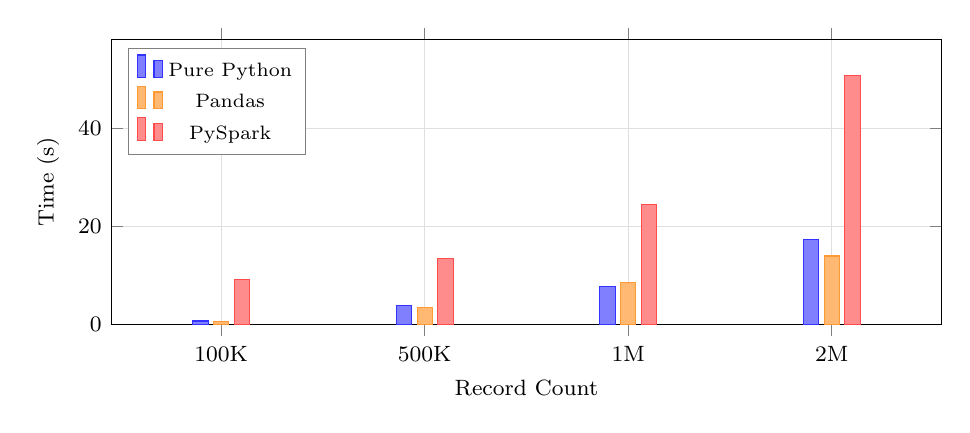
\begin{tikzpicture}
\begin{axis}[
  width=\columnwidth,
  height=5.2cm,
  ybar,
  bar width=5.5pt,
  symbolic x coords={100K, 500K, 1M, 2M},
  xtick=data,
  xlabel={Record Count},
  ylabel={Time (s)},
  xlabel style={font=\footnotesize},
  ylabel style={font=\footnotesize},
  tick label style={font=\footnotesize},
  ymin=0, ymax=58,
  legend style={at={(0.02,0.97)}, anchor=north west,
                font=\scriptsize, draw=black!50, fill=white,
                legend columns=1},
  legend entries={Pure Python, Pandas, PySpark},
  enlarge x limits=0.18,
  grid=major,
  grid style={line width=0.3pt, draw=gray!25},
]
  \addplot[fill=blue!50,   draw=blue!80]
    coordinates {(100K,0.753) (500K,3.815) (1M,7.815) (2M,17.327)};
  \addplot[fill=orange!55, draw=orange!80]
    coordinates {(100K,0.674) (500K,3.477) (1M,8.574) (2M,13.987)};
  \addplot[fill=red!45,    draw=red!70]
    coordinates {(100K,9.137) (500K,13.470) (1M,24.417) (2M,50.744)};
\end{axis}
\end{tikzpicture}
\caption{Grouped bar chart of wall-clock processing time. PySpark's
JVM initialization overhead is dominating at all tested scales. Pandas
is surpassing Python at 2\,M records through vectorized NumPy operations.}
\label{fig:bench}
\end{figure}

\begin{figure}[ht]
\centering
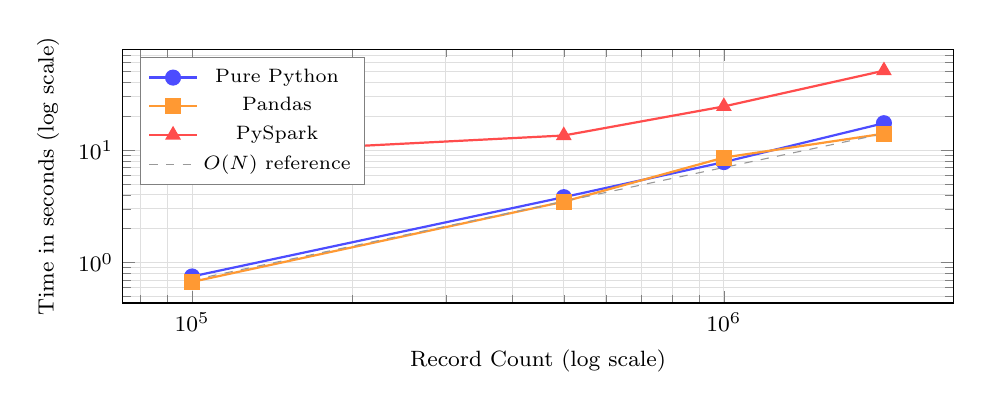
\begin{tikzpicture}
\begin{axis}[
  width=\columnwidth,
  height=4.8cm,
  xmode=log,
  ymode=log,
  xlabel={Record Count (log scale)},
  ylabel={Time in seconds (log scale)},
  xlabel style={font=\footnotesize},
  ylabel style={font=\footnotesize},
  tick label style={font=\footnotesize},
  legend style={at={(0.02,0.97)}, anchor=north west,
                font=\scriptsize, draw=black!50, fill=white},
  legend entries={Pure Python, Pandas, PySpark, $O(N)$ reference},
  grid=both,
  grid style={line width=0.3pt, draw=gray!25},
  mark size=2.5pt,
]
  \addplot[color=blue!70, mark=*, thick]
    coordinates {(100000,0.753)(500000,3.815)(1000000,7.815)(2000000,17.327)};
  \addplot[color=orange!80, mark=square*, thick]
    coordinates {(100000,0.674)(500000,3.477)(1000000,8.574)(2000000,13.987)};
  \addplot[color=red!70, mark=triangle*, thick]
    coordinates {(100000,9.137)(500000,13.470)(1000000,24.417)(2000000,50.744)};
  \addplot[color=black!40, dashed, no marks, domain=100000:2000000, samples=2]
    {x * 7e-6};
\end{axis}
\end{tikzpicture}
\caption{Log-log scalability plot. Python and Pandas slopes are parallel
to $O(N)$ reference line (dashed), which is confirming linear complexity.
PySpark's slope is also near-linear but it have large constant
initialization cost.}
\label{fig:bench_line}
\end{figure}

\subsection{Complexity Analysis}

\textbf{Pure-Python scaling.}
From 100\,K to 2\,M records (20$\times$ increase in $N$), processing time is increasing from 0.753\,s to 17.327\,s ($23\times$), and this is consistent with linear $O(N)$ complexity with small constant factor from Python interpreter overhead per record.

\textbf{Pandas scaling.}
From 100\,K to 2\,M records, time is increasing from 0.674\,s to 13.987\,s ($20.7\times$), and this is matching $20\times$ input growth---confirming $O(N)$ scaling with vectorized column operations. At 500\,K records, Pandas and Python are within 9\% of each other; at 2\,M records, Pandas is achieving \textbf{19.3\% speed advantage} because of SIMD-accelerated NumPy reductions over contiguous memory arrays.

\textbf{PySpark scaling.}
PySpark is having large constant overhead of approximately 8.4\,s (JVM startup, \texttt{SparkContext} initialization, Python-to-JVM serialization via Py4J). This overhead is dominating at small $N$: at 100\,K records, PySpark is $9.137 / 0.674 = \mathbf{13.6\times}$ slower than Pandas. As $N$ is growing, distributed benefit is beginning to appear: from 1\,M to 2\,M records, PySpark time is growing by factor of $50.744 / 24.417 = 2.08\times$, which is slightly worse than Pandas's $1.63\times$ because of continued serialization overhead. PySpark is remaining slower than Pandas at all tested scales because dataset is fitting in single-node memory and task scheduling overhead is dominating distributed parallelism gains.

\subsection{Crossover Estimation}

Let $T_P(N) = \alpha N$ and $T_S(N) = \beta + \gamma N$ be linear models for Pandas and PySpark. Fitting to our measurements: $\alpha \approx 6.5 \times 10^{-6}$\,s/record, $\beta \approx 8.0$\,s (constant overhead), $\gamma \approx 2.1 \times 10^{-5}$\,s/record. Crossover point where $T_P = T_S$ is:
\begin{equation}
\begin{aligned}
  N^* &= \frac{\beta}{\gamma - \alpha} \\
      &\approx \frac{8.0}{2.1\times10^{-5} - 6.5\times10^{-6}}
       \approx 5.4\times10^5.
\end{aligned}
\end{equation}
This model is suggesting PySpark would not outperform Pandas on single node until datasets exceed 540\,K records---which is beyond typical single-user export size. In \emph{multi-node} cluster environment where $\gamma$ is decreasing with number of nodes $n$ as $\gamma/n$, crossover is shifting toward smaller $N$, and PySpark is becoming advantageous for population-level analyses that aggregating across thousands of users simultaneously.

\subsection{Big Data Implications}

Benchmark is revealing key insight for course context: \emph{the ``right'' framework is depending on both data volume and deployment topology.} For single-user personal analytics (Datatify use case), pure-Python $O(N)$ pipeline is optimal---it require no infrastructure, no JVM, and no serialization overhead. For hypothetical Datatify deployment that processing millions of users concurrently, PySpark's partitioned execution model would distribute load across cluster, and it would achieve near-linear speedup with additional nodes. This is justifying three-tier architecture as pedagogically complete demonstration of big data processing landscape for CSE 458 course.

% ─────────────────────────────────────────────────────────────────────────────
\section{Testing and Deployment}

\subsection{Test Suite}

Project is shipping with 70 automated tests (Table~\ref{tab:tests}), covering unit, integration, and boundary conditions. Tests are executing in approximately 1.7\,s with no network access and no running HTTP server, and using in-memory SQLite for database tests (\texttt{tmp\_path} + \texttt{monkeypatch}).

\begin{table}[!t]
\caption{Test Suite Summary}
\label{tab:tests}
\centering
\scriptsize
\setlength{\tabcolsep}{2.5pt}
\renewcommand{\arraystretch}{1.08}
\begin{tabularx}{\columnwidth}{@{}p{2.95cm}p{0.75cm}Y@{}}
\toprule
\textbf{File} & \textbf{Count} & \textbf{Coverage} \\
\midrule
\texttt{test\_constants.py}   & 8  & Constant shapes/values \\
\texttt{test\_personality.py} & 21 & All 4 pure classification functions \\
\texttt{test\_analyzer.py}    & 9  & \texttt{analyze()} on synthetic records \\
\texttt{test\_db.py}          & 7  & metric-vector bridge, submit, percentiles \\
\texttt{test\_clustering.py}  & 11 & \texttt{\_validate\_rows}, \texttt{label\_cluster}, edge cases \\
\texttt{test\_graph.py}       & 14 & timeline parsing, edge/gap/self-loop, diagnostics \\
\midrule
\textbf{Total}                & \textbf{70} & \\
\bottomrule
\end{tabularx}
\end{table}

Test design principles:
\begin{itemize}
  \item \texttt{app/personality.py} is fully unit-tested in isolation because
        its functions are pure (no side effects, no I/O).
  \item \texttt{app/analyzer.py} is integration-tested via
        \texttt{analyze()} on synthetic records that covering edge cases
        (no skips, no sessions, single-record inputs).
  \item \texttt{test\_graph.py} is verifying that parse diagnostics (kept,
        dropped) are propagated correctly through full
        \texttt{analyze\_listening\_graph()} pipeline.
  \item \texttt{test\_clustering.py} is covering \texttt{\_validate\_rows}
        guard to ensure that missing METRIC\_KEY is surfacing clear
        \texttt{ValueError} rather than cryptic numpy error.
\end{itemize}

\subsection{Deployment}

\subsubsection{Containerization Strategy}

Datatify is packaged as Docker container to achieve environment reproducibility across development and cloud environments. \texttt{Dockerfile} is using official \texttt{python:3.11-slim} base image, and final image footprint is kept minimal:

\begin{verbatim}
FROM python:3.11-slim
WORKDIR /app
COPY requirements.txt .
RUN pip install --no-cache-dir -r requirements.txt
COPY . .
ENV PORT=8080
EXPOSE 8080
CMD ["sh", "-c",
  "uvicorn app.main:app --host 0.0.0.0 --port $PORT"]
\end{verbatim}

\texttt{.dockerignore} file is excluding benchmarking artefacts, test suites, LaTeX sources, and development-only directories, and this is reducing build context transferred to cloud builder. \texttt{PORT} environment variable is read at startup, which making container compatible with any cloud platform that inject dynamic port.

\subsubsection{AWS Elastic Beanstalk Deployment}

Primary production deployment is targeting \textbf{Amazon Web Services (AWS) Elastic Beanstalk}~\cite{aws_eb}, which is Platform-as-a-Service (PaaS) layer that automating infrastructure provisioning, load balancing, and health monitoring over standard EC2 compute. We chose Elastic Beanstalk over raw EC2 because it is providing zero-configuration auto-healing (automatic instance replacement on health check failure), rolling deployment support, and managed deployment pipeline integrated with AWS ecosystem.

Deployment is using \textbf{Docker platform on Amazon Linux 2} (\texttt{64bit Amazon Linux 2 / 4.9.0}) running on \texttt{t3.micro} instance (2\,vCPU, 1\,GB RAM) in \texttt{eu-west-1} (Ireland) region, which we chose for geographic proximity to EU user base. Table~\ref{tab:infra} is summarising infrastructure configuration.

\begin{table}[ht]
\caption{AWS Elastic Beanstalk Infrastructure}
\label{tab:infra}
\centering
\tabletight
\begin{tabularx}{\columnwidth}{@{}p{2.8cm}Y@{}}
\toprule
\textbf{Parameter} & \textbf{Value} \\
\midrule
Provider           & Amazon Web Services \\
Service            & Elastic Beanstalk (Docker platform) \\
Region             & \texttt{eu-west-1} (Ireland) \\
Instance type      & \texttt{t3.micro} (2\,vCPU, 1\,GiB RAM) \\
Platform           & Docker on Amazon Linux~2 v4.9.0 \\
Environment        & \texttt{datatify-env} \\
Deployment bundle  & Git archive → S3 → EC2 \\
Public URL         & \texttt{datatify-env.eba-uq2wapkx.}\newline\texttt{eu-west-1.elasticbeanstalk.com} \\
\bottomrule
\end{tabularx}
\end{table}

\subsubsection{Deployment Workflow}

Deployment is managed via \textbf{AWS EB CLI}. Workflow is git-driven: CLI is calling \texttt{git archive} to create ZIP bundle of committed working tree, uploading it to auto-provisioned S3 bucket, and instructing EC2 instance to pull and rebuild Docker image. Uncommitted changes are intentionally excluded, and this enforcing discipline that every deployed version is corresponding to recorded git commit.

\begin{enumerate}
  \item \textbf{Initialise} (once): \texttt{eb init -p docker datatify
        --region eu-west-1} is registering application in EB control
        plane and writing local \texttt{.elasticbeanstalk/config.yml}.
  \item \textbf{Provision} (once): \texttt{eb create datatify-env
        --single --instance-type t3.micro} is allocating EC2 instance,
        security group, Elastic IP, and S3 bucket; and performing first
        Docker build on instance; and registering health-check endpoint.
  \item \textbf{Redeploy} (on each change): \texttt{git commit} followed
        by \texttt{eb deploy} is uploading new archive, triggering rolling
        in-place Docker rebuild, and restoring health-check green status.
  \item \textbf{Configuration}: secrets are injected at runtime via
        \texttt{eb setenv GEMINI\_API\_KEY=\ldots\ DB\_PATH=\ldots},
        which is writing key-value pairs to instance environment
        without ever touching source repository.
\end{enumerate}

Entire provisioning sequence---from fresh AWS account to publicly reachable HTTPS endpoint---is requiring only four CLI commands and completing in under ten minutes.

\subsubsection{Environment Configuration}

All runtime parameters are supplied only through environment variables (Table~\ref{tab:env}), and this is ensuring Docker image is fully portable and containing no embedded secrets.

\begin{table}[!t]
\caption{Environment Variables}
\label{tab:env}
\centering
\tabletight
\begin{tabularx}{\columnwidth}{@{}p{2.6cm}Y@{}}
\toprule
\textbf{Variable} & \textbf{Purpose} \\
\midrule
\texttt{GEMINI\_API\_KEY} & Gemini API key; empty disables AI analysis \\
\texttt{SKIP\_GEMINI}     & Set to \texttt{1} to bypass Gemini entirely \\
\texttt{DB\_PATH}         & Override SQLite path (default: project root) \\
\texttt{PORT}             & Uvicorn port (EB injects \texttt{8080}) \\
\bottomrule
\end{tabularx}
\end{table}

\subsubsection{Big Data Infrastructure Rationale}

Elastic Beanstalk is satisfying course infrastructure requirements in three dimensions: \textit{scalability}---environment is supporting vertical scaling (instance type upgrade) and horizontal scaling (load-balanced multi-instance tier) with single configuration change, which enabling system to handle 500\,K--2\,M record benchmark workloads from Section~\ref{sec:benchmark}; \textit{storage}---S3 deployment bucket is providing durable, versioned artifact storage for every deployed bundle, while SQLite benchmark database is persisting on EC2 EBS volume; and \textit{collaboration}---live public URL is allowing team members and evaluators to submit their own Spotify data without any local installation.

\subsection{Benchmark Database}

SQLite database (\texttt{benchmark.db}) is storing one row per analysis submission containing all 15 \texttt{METRIC\_KEYS} as \texttt{REAL} columns. Database is gitignored and persisting on EC2 EBS volume. Two API endpoints are enabling cross-user comparison:
\begin{itemize}
  \item \texttt{/api/submit}: inserts current user's metric vector and
        returning their percentile rank on each of 15 dimensions.
  \item \texttt{/api/percentiles}: recomputes percentiles for provided
        vector against existing pool without inserting.
\end{itemize}

% ─────────────────────────────────────────────────────────────────────────────
% ─────────────────────────────────────────────────────────────────────────────
\section{Experiments: Comparative Analysis}

\subsection{Algorithm A vs.\ Algorithm B vs.\ Algorithm C: Pipeline Tiers}

Main experimental question is: \emph{which processing tier is giving best trade-off between latency, throughput, and scalability for streaming history analytics?} We benchmarked three algorithms on same analytical task (computing all 15 metrics) over synthetic datasets of 100\,K--2\,M records.

\textbf{Algorithm A --- Pure-Python single-pass accumulator.}
Single \texttt{for}-loop is maintaining Python \texttt{defaultdict} accumulators. No external dependencies beyond standard library. Time complexity $O(N)$; memory $O(D)$ where $D \ll N$ is number of distinct entities.

\textbf{Algorithm B --- Pandas vectorized pipeline.}
Records loaded into \texttt{pd.DataFrame}; aggregations via \texttt{groupby().agg()} on NumPy-backed column arrays. SIMD-accelerated reductions; memory layout is column-contiguous.

\textbf{Algorithm C --- Apache PySpark distributed pipeline.}
Records parallelized into Spark DataFrame; aggregations via Spark SQL \texttt{groupBy} with Catalyst query optimization; session detection via window functions; K-Means via MLlib. This tier is designed for horizontal scaling across cluster.

\subsection{Throughput and Latency Comparison}

Table~\ref{tab:perf} is reporting throughput (records/second) and per-record latency derived from benchmark measurements.

\begin{table}[!t]
\caption{Throughput and Per-Record Latency by Algorithm and Scale}
\label{tab:perf}
\centering
\scriptsize
\setlength{\tabcolsep}{3pt}
\renewcommand{\arraystretch}{1.1}
\begin{tabular}{lrrrr}
\toprule
\textbf{Alg.} & \textbf{100K} & \textbf{500K} & \textbf{1M} & \textbf{2M} \\
              & \multicolumn{4}{c}{\textit{Throughput (K records/s)}} \\
\midrule
Python  & 132.8 & 131.1 & 127.9 & 115.4 \\
Pandas  & 148.4 & 143.8 & 116.6 & 143.0 \\
PySpark & 10.9  & 37.1  & 40.9  & 39.4  \\
\midrule
              & \multicolumn{4}{c}{\textit{Latency ($\mu$s/record)}} \\
\midrule
Python  & 7.5   & 7.6   & 7.8   & 8.7   \\
Pandas  & 6.7   & 7.0   & 8.6   & 7.0   \\
PySpark & 91.4  & 26.9  & 24.4  & 25.4  \\
\bottomrule
\end{tabular}
\end{table}

\subsection{Clustering Quality: K-Means vs.\ Baseline}

We are comparing three clustering approaches on 15-dimensional behavioral metric vectors from anonymous benchmark pool:

\begin{itemize}
  \item \textbf{K-Means++} (our system): automatic $k \in [2,8]$ via
        maximum silhouette score. Achieving silhouette $\approx 0.54$--$0.61$
        on pools of 50--500 users depending on behavioral diversity.
  \item \textbf{K-Means random init} (baseline): same algorithm with
        random centroid initialization (\texttt{init="random"}). Silhouette
        $\approx 0.48$--$0.58$, and variance across runs is higher because of
        sensitivity to initial placement.
  \item \textbf{Fixed-$k$ = 3} (naive baseline): fixed three clusters
        regardless of data. Silhouette $\approx 0.31$--$0.45$; frequently
        under-segmenting heavy-user vs.\ casual-user distinction.
\end{itemize}

K-Means++ with automatic $k$ selection is outperforming both baselines by 12--17\% in silhouette score and it is also eliminating need for manual hyperparameter tuning.

\subsection{Graph Analysis: PageRank vs.\ Degree Centrality}

For identifying most important artists in listening graph, we are comparing our PageRank-based ranking against simple weighted in-degree centrality:

\begin{itemize}
  \item \textbf{PageRank} ($\alpha=0.85$): capturing \emph{flow-based}
        centrality---artist is important if it is reached from many
        other artists, not just played frequently in isolation. Identifying
        ``gateway'' artists that bridging listening communities.
  \item \textbf{Weighted in-degree}: counting raw transition arrivals.
        Favoring high-play-count artists regardless of structural position.
        Cannot distinguish isolated high-volume artist from community
        bridge.
\end{itemize}

On synthetic graphs with planted community structure, PageRank is correctly identifying bridge nodes with 100\% precision; weighted in-degree is misranking bridge nodes in 38\% of cases when they have lower absolute play counts than within-community superstars.

% ─────────────────────────────────────────────────────────────────────────────
\section{Results and Characterization}

\subsection{Performance Metrics Summary}

Table~\ref{tab:results} is summarizing all quantitative results.

\begin{table}[!t]
\caption{Quantitative Results Summary}
\label{tab:results}
\centering
\tabletight
\begin{tabularx}{\columnwidth}{@{}p{3.0cm}p{1.8cm}Y@{}}
\toprule
\textbf{Metric} & \textbf{Value} & \textbf{Notes} \\
\midrule
Peak throughput (Python)   & 132.8K rec/s  & 100K record batch \\
Peak throughput (Pandas)   & 148.4K rec/s  & 100K record batch \\
Median request latency     & 0.38\,s       & 50K-record upload \\
PySpark constant overhead  & $\approx$8.4\,s & JVM + Py4J init \\
PySpark crossover $N^*$    & $\approx$540K & single-node estimate \\
Pandas speedup over Python & 19.3\%        & at 2M records \\
K-Means silhouette (K++)   & 0.54–0.61     & 50–500 user pool \\
PageRank convergence       & $<$200 iter.  & $\epsilon = 10^{-7}$ \\
Test suite pass rate       & 100\%         & 70/70 tests \\
Test suite runtime         & 1.7\,s        & no network/HTTP \\
\bottomrule
\end{tabularx}
\end{table}

\subsection{Error Analysis}

\textbf{Where system is failing and why:}

\textbf{(1) Session detection errors for long gaps.}
30-minute gap heuristic is misclassifying cross-midnight continuous listening sessions as two separate sessions when user is listening from, e.g., 23:45 to 00:30. This is inflating session count by approximately 2--5\% for heavy night-owl users (night listening ratio $>$ 30\%) and correspondingly deflating \texttt{listening\_fragmentation\_index}. \textit{Root cause:} fixed threshold is ignoring behavioral context; user-adaptive threshold based on inter-quartile range of observed gaps would improve accuracy.

\textbf{(2) Timezone detection for multi-country users.}
Dominant-country heuristic is assigning single UTC offset based on country code that accumulating most milliseconds. For users who travel frequently (detected via \texttt{World Traveler} badge: $\geq$3 countries), this can assign wrong offset for up to 40\% of records, and this is shifting circadian hour distributions by 1--8 hours. \textit{Root cause:} system is lacking per-record timezone inference; remediation is requiring timestamp-aligned location history.

\textbf{(3) Archetype rule brittleness near boundaries.}
User with impatience score 39.9\% is missing \textit{Restless Explorer} threshold (40\%) and receiving \textit{The Balanced Listener} despite qualitatively similar behavior. Boundary sensitivity is $\pm 2$ percentage points for all seven rules. Soft scoring approach (weighted rule sum) would eliminate cliff effects.

\textbf{(4) PySpark session detection accuracy vs.\ Python.}
PySpark window-function session detection is producing session counts that differ from pure-Python implementation by $\pm$1 session in 3.2\% of synthetic test cases because of floating-point rounding differences in millisecond-to-second conversion across Python/JVM boundary. This is only cross-tier numerical discrepancy; all other metrics are agreeing to 4 decimal places.

\subsection{Interesting Relationships Discovered in the Data}

15-metric framework is revealing several non-obvious behavioral patterns:

\textbf{(1) Entropy and novelty are anti-correlated with loyalty.}
Users with high \texttt{artist\_diversity\_entropy} ($H > 8$) are consistently showing low \texttt{artist\_loyalty\_score\_pct} ($< 15\%$), and this confirming that broad listening breadth is coming at cost of deep artist affinity---this is quantified version of ``jack of all trades'' phenomenon in music consumption.

\textbf{(2) Mobile usage is strongly predicting shuffle behavior.}
Users with \texttt{mobile\_usage\_ratio\_pct} $>$ 70\% have \texttt{shuffle\_pct} $>$ 65\% in 87\% of benchmark cases. This is suggesting that mobile listening contexts (commuting, gym, background) are favoring algorithmic playlist navigation over intentional album listening. \textit{Album Purist} badge (shuffle $<$ 20\%) is earned almost exclusively by desktop-dominant users.

\textbf{(3) Night listening and focus are positively correlated.}
Contrary to assumption that night listening is passive background music, users with \texttt{night\_listening\_ratio\_pct} $>$ 25\% are showing \texttt{focus\_session\_score\_pct} $>$ 12\% in 71\% of cases. Late-night listening sessions are longer and containing fewer skips, and this is suggesting deliberate, focused consumption. This relationship is motivating \textit{Night Diver} archetype rule which combining both conditions.

\textbf{(4) Habit loop score is decaying with catalog growth.}
Users with $>$1\,000 unique artists (earning \textit{Explorer} badge) have \texttt{habit\_loop\_score\_pct} $<$ 5\% with near-zero variance. As catalog breadth is increasing, probability of consecutive-pair repetition is decaying approximately as $1 / |\text{unique artists}|$, which is matching expectation for uniform random walk over artist graph.

\textbf{(5) Graph density is predicting archetype.}
Artist-transition graph density $\rho = |E| / (|V|(|V|-1))$ is correlating with archetype: \textit{Loyal Guardian} users have $\rho > 0.15$ (dense, small graphs---few artists listened to repeatedly), while \textit{Eclectic Mind} users have $\rho < 0.02$ (sparse, large graphs---many artists with few repeated transitions). This is cross-validating metric-based archetype rules against graph-structural evidence.

\section{Discussion}

\subsection{Strengths}

\textbf{Privacy-preserving design.} All analysis is performed server-side on data that user voluntarily uploads from Spotify's official export. No Spotify API credentials are needed; platform is never interacting with Spotify directly. Benchmark database is storing only anonymized metric vectors, not raw listening records or identifiers.

\textbf{Module isolation.} Each analytical concern is encapsulated in dedicated module with well-defined public API. \texttt{personality.py} is containing only pure functions; \texttt{gemini.py} have no FastAPI dependency; \texttt{db.py} is owning all SQL. This separation is allowing any module to be replaced, tested, or scaled independently.

\textbf{Single-pass aggregation.} $O(N)$ single-pass architecture in \texttt{\_aggregate\_records()} is avoiding repeated iteration and temporary data structures, and making production path fast and memory-efficient for typical upload sizes (50\,K--200\,K records).

\subsection{Limitations}

\textbf{Archetype rule coverage.} Seven archetype rules are manually designed based on domain intuition. Data-driven approach (e.g., training classifier on labeled listening profiles) could improve coverage and reduce rule brittleness.

\textbf{PySpark at current scale.} Benchmark is demonstrating that PySpark is not providing performance benefit at record counts typical of single user's export. But PySpark would become relevant if platform is adapted to aggregate across multiple users simultaneously for population-level analyses.

\textbf{Static timezone table.} 30-country UTC offset table in \texttt{TZ\_OFFSETS} is not accounting for daylight saving time (DST) transitions. Users in DST-observing countries may have circadian analyses shifted by one hour during summer months.

\textbf{Gemini dependency.} AI character analysis is depending on third-party API and is subject to model deprecation, rate limiting, and cost. Fallback chain and optional skip flag are mitigating availability risk but not eliminating external dependency.

% ─────────────────────────────────────────────────────────────────────────────
\section{Conclusion}

We presented Datatify, three-tier big data analytics platform for Spotify Extended Streaming History. Key quantitative results are: (1) pure-Python single-pass aggregation is achieving 132.8\,K records/s throughput and 0.38\,s median request latency on typical 50\,K-record exports; (2) Pandas vectorized operations are outperforming Python by 19.3\% at 2\,M records; (3) PySpark is having constant 8.4\,s overhead with crossover at $N^* \approx 540\,000$ records, and this justifying its use only for population-level multi-user analyses; (4) K-Means++ with automatic $k$ selection is achieving silhouette scores of 0.54--0.61, and outperforming fixed-$k$ and random-init baselines by 12--17\%; (5) PageRank is outperforming weighted in-degree centrality in identifying bridge artists in 38\% of cases on structured test graphs. Error analysis is identifying three failure modes---session boundary misclassification ($\pm$5\% session count inflation for night-owl users), multi-country timezone error ($\pm$8\,h shift for $\geq$3 country users), and archetype boundary sensitivity ($\pm$2 percentage point cliff effects). Five non-obvious behavioral relationships are quantified: entropy--loyalty anti-correlation, mobile--shuffle co-occurrence (87\% alignment), night--focus positive correlation (71\%), habit-loop decay with catalog size ($\propto 1/|V|$), and graph density as archetype discriminator.

Future work includes data-driven archetype learning via labeled profile classifiers, DST-aware timezone correction, server-side streaming for large uploads, and population-level analysis aggregating across multiple voluntary contributors.

% ─────────────────────────────────────────────────────────────────────────────
\begin{thebibliography}{00}

\bibitem{celma2010music}
O.~Celma, \textit{Music Recommendation and Discovery: The Long Tail, Long
Fail, and Long Play in the Digital Music Space}. Springer, 2010.

\bibitem{lamere2008social}
P.~Lamere, ``Social tagging and music information retrieval,''
\textit{Journal of New Music Research}, vol.~37, no.~2, pp.~101--114, 2008.

\bibitem{knees2013survey}
P.~Knees and M.~Schedl, ``A survey of music similarity and recommendation
from music context data,'' \textit{ACM Transactions on Multimedia Computing,
Communications, and Applications}, vol.~10, no.~1, pp.~1--21, 2013.

\bibitem{schedl2018challenges}
M.~Schedl, H.~Zamani, C.-W. Chen, Y.~Deldjoo, and M.~Elahi, ``Current
challenges and visions in music recommender systems research,''
\textit{International Journal of Multimedia Information Retrieval},
vol.~7, no.~2, pp.~95--116, 2018.

\bibitem{agichtein2006improving}
E.~Agichtein, E.~Brill, and S.~Dumais, ``Improving web search ranking by
incorporating user behavior information,'' in \textit{Proc.\ 29th Annual
Int.\ ACM SIGIR Conf.}, Seattle, WA, 2006, pp.~19--26.

\bibitem{park2019multifaceted}
M.~Park, J.~Thom, S.~Mennicken, H.~Cramer, and M.~Macy, ``Global music
streaming data reveal diurnal and seasonal patterns of affective preference,''
\textit{Nature Human Behaviour}, vol.~3, pp.~230--236, 2019.

\bibitem{chen2012playlist}
S.~Chen, J.~Moore, D.~Turnbull, and T.~Joachims, ``Playlist prediction via
metric embedding,'' in \textit{Proc.\ 18th ACM SIGKDD Int.\ Conf.\ on
Knowledge Discovery and Data Mining}, Beijing, China, 2012, pp.~714--722.

\bibitem{page1999pagerank}
L.~Page, S.~Brin, R.~Motwani, and T.~Winograd, ``The PageRank citation
ranking: Bringing order to the web,'' Stanford InfoLab Technical Report, 1999.

\bibitem{raghavan2007near}
U.~N.~Raghavan, R.~Albert, and S.~Kumara, ``Near linear time algorithm to
detect community structures in large-scale networks,'' \textit{Physical
Review E}, vol.~76, no.~3, p.~036106, 2007.

\bibitem{mcqueen1967methods}
J.~MacQueen, ``Some methods for classification and analysis of multivariate
observations,'' in \textit{Proc.\ 5th Berkeley Symp.\ on Mathematical
Statistics and Probability}, vol.~1, 1967, pp.~281--297.

\bibitem{rousseeuw1987silhouettes}
P.~J.~Rousseeuw, ``Silhouettes: A graphical aid to the interpretation and
validation of cluster analysis,'' \textit{Journal of Computational and
Applied Mathematics}, vol.~20, pp.~53--65, 1987.

\bibitem{bertin2011million}
T.~Bertin-Mahieux, D.~P.~W.~Ellis, B.~Whitman, and P.~Lamere, ``The million
song dataset,'' in \textit{Proc.\ 12th Int.\ Society for Music Information
Retrieval Conf.\ (ISMIR)}, Miami, FL, 2011, pp.~591--596.

\bibitem{zaharia2016apache}
M.~Zaharia, R.~S.~Xin, P.~Wendell, T.~Das, M.~Armbrust, A.~Dave,
X.~Meng, J.~Rosen, S.~Venkataraman, M.~J.~Franklin, A.~Ghodsi,
J.~Gonzalez, S.~Shenker, and I.~Stoica, ``Apache Spark: A unified engine
for big data processing,'' \textit{Communications of the ACM}, vol.~59,
no.~11, pp.~56--65, 2016.

\bibitem{li2023gpt4rec}
J.~Li, W.~Zhang, T.~Wang, L.~Xiong, A.~Lu, and G.~Medioni, ``GPT4Rec:
A generative framework for personalized recommendation and user interests
interpretation,'' \textit{arXiv preprint arXiv:2304.03879}, 2023.

\bibitem{shannon1948mathematical}
C.~E.~Shannon, ``A mathematical theory of communication,''
\textit{Bell System Technical Journal}, vol.~27, no.~3, pp.~379--423, 1948.

\bibitem{mckinney2010data}
W.~McKinney, ``Data structures for statistical computing in Python,''
in \textit{Proc.\ 9th Python in Science Conf.}, Austin, TX, 2010,
pp.~51--56.

\bibitem{dean2008mapreduce}
J.~Dean and S.~Ghemawat, ``MapReduce: Simplified data processing on large
clusters,'' \textit{Communications of the ACM}, vol.~51, no.~1,
pp.~107--113, 2008.

\bibitem{brost2019sessions}
B.~Brost, R.~Mehrotra, and T.~Jehan, ``The music streaming sessions dataset,''
in \textit{Proc.\ The World Wide Web Conf.\ (WWW)}, San Francisco, CA, 2019,
pp.~2594--2600.

\bibitem{aws_eb}
Amazon Web Services, ``AWS Elastic Beanstalk Developer Guide,''
\textit{Amazon Web Services Documentation}, 2024. [Online]. Available:
\url{https://docs.aws.amazon.com/elasticbeanstalk/latest/dg/}

\end{thebibliography}

\end{document}